\section{Finite Element Modeling}

When performing optimization to find designs, numerous designs must be analyzed and evaluated for fitness. In some cases, these designs and their fitness functions can be modeled using closed form equations. In the many cases, however, the designs are complex enough that finding closed form models of their behavior is infeasible. In the case that no closed form solutions can be found, numerical analysis can offer an alternative method of evaluating for fitness. 

For this study, numerical analysis in the form of Finite Element Modeling was chosen as the method for evaluating the designs for fitness. Each design and load case each are represented as slight modifications to a basic model file containing the fixed geometry and ``starting" parameters for the design and loading variables.  \todo{Do I need to summarize the basics of finite element modeling?}

This study makes exclusive use of quadrilaterial shell elements, known to NASTRAN as \codeword{CQUAD4} elements. These elements are 2-dimensional, but do model deformation in all thee dimensions. However, an important assumption made by using these elements is that the entire thickness of the plate distributes the stress applied to the element equally. This implies that deformations in the thickness direction cannot be modeled this way. For example, if a plate can buckle or bend through its thickness this type of element would not be suitable. This model makes use of these elements for the beam flanges, but the elements are oriented to be coplanar with the beam web. This means the flange width is modeled as plate thickness. This orientation will not detect local flange effects such as buckling or local bending. However, this study is primarily concerned with failure of the gross section. Due to the system geometry, these stresses are negligable and therefore the model's inability to properly model them does not appreciably affect the accuracy of this model. This modeling strategy also has the advantage of simplifying the alteration of the flange thickness programmatically. 

\subsection{Selected Model}

\begin{figure}
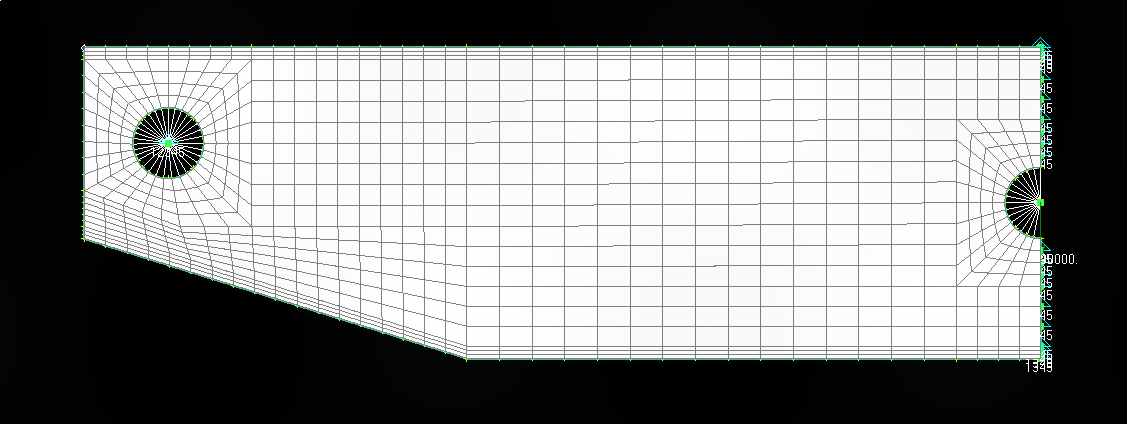
\includegraphics[width=\textwidth]{img/mesh_geom.png}
\caption{Mesh Geometry as shown in Siemens Femap}
\label{img:mesh_geom}
\end{figure}

The model developed for the example problem considered in this work is shown in figure \ref{img:mesh_geom}. This model was developed using the dimensional data shown in figure \ref{img:dim_beam}. As shown, the model consists of several regions, all of which are modeled using \codeword{CQUAD4} elements. The regions that are of importance for this study are: 

\begin{enumerate}
  \item The top flange
  \item The bottom flange
  \item The web
  \item A thickened region surrounding the hoist mounting lug
  \item A thickened region surrounding the load mounting lug. 
\end{enumerate}

\begin{figure}
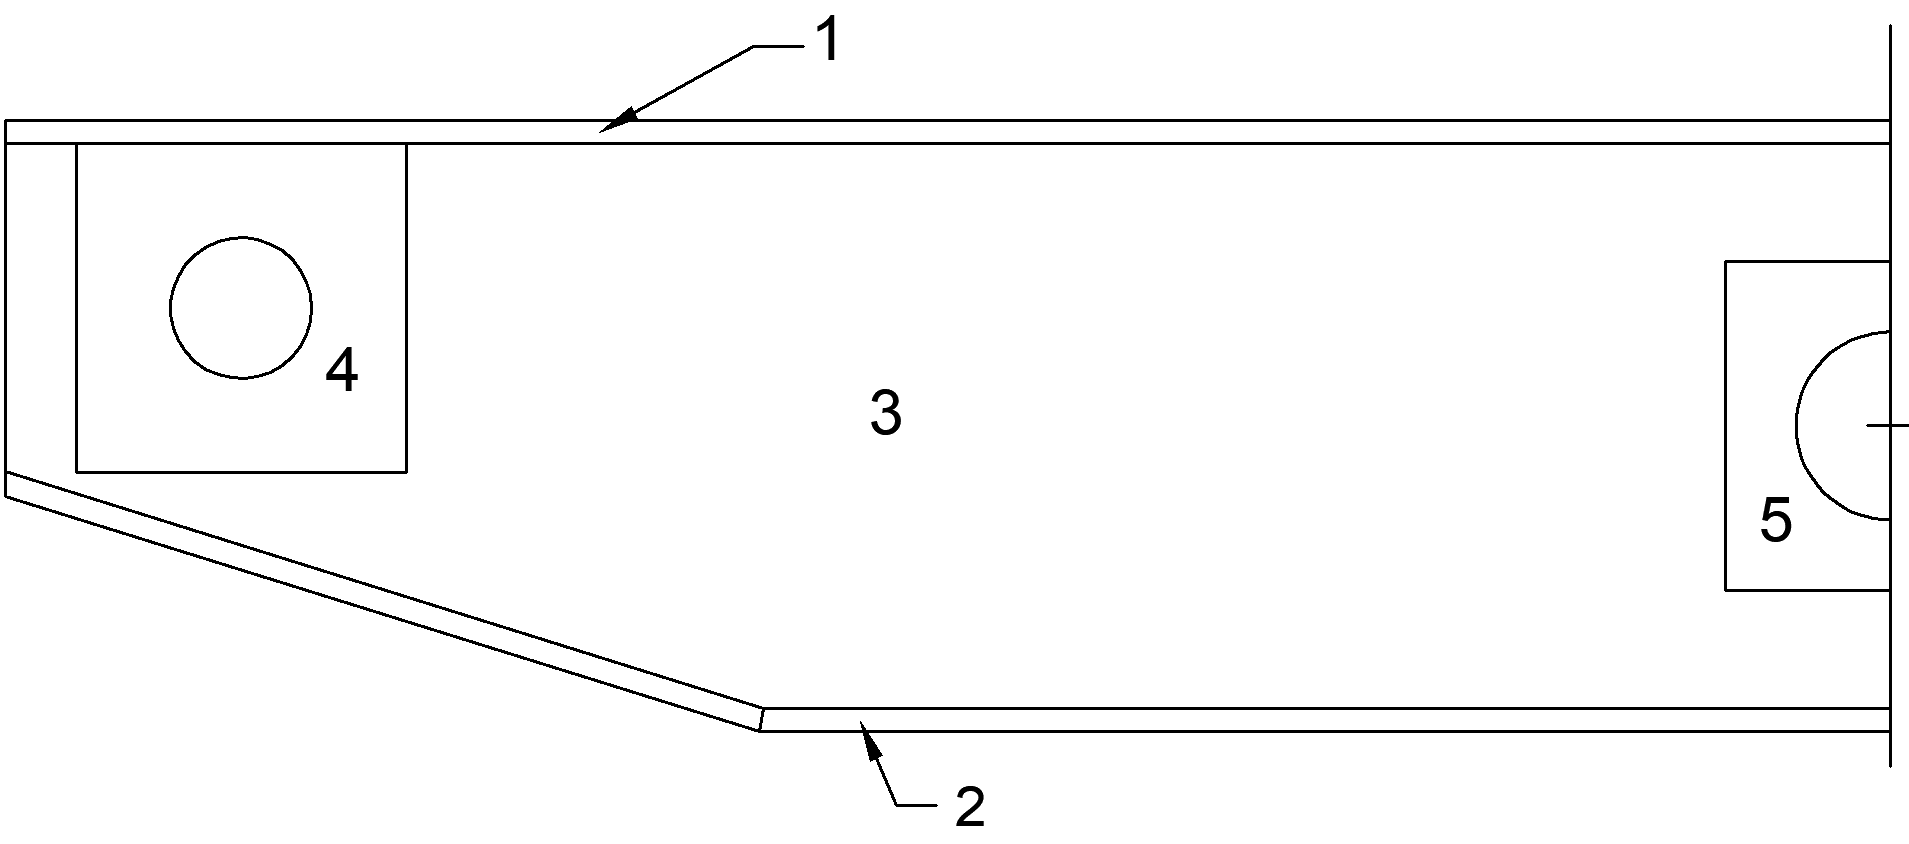
\includegraphics[width=\textwidth]{img/numbered_geom.png}
\caption{Diagram of modeled beam showing region numbers}
\label{img:num_geom}
\end{figure}

Figure \ref{img:num_geom} shows the named regions as they correspond to portions of the model/drawing. 

Also worth noting is that this model is a partial representation of the whole beam. As the example beam in figure \ref{img:basic_beam} shows, the beam features symmetry along the front view. Due to the typical construction of these beams, they also exhibit symmetry along the top view as well. Because of this, the model presented is only one quarter of the complete beam. To account for this, constraints are imposed along the symmetry cut that simulate the remainder of the beam. These constraints can be seen in figure \ref{img:mesh_geom} as symbols along the right edge of the diagram. These constraints are along model axes 1, 3, 4, and 5. This equates to constraining X and Z translation, as well as X and Y rotations. This simulates a moment bearing connection at the center of the beam. This is a commonly accpeted way of simulating symmetry in NASTRAN\todo{Needs Citation}. 

